\chapter{Verfahrensbeschreibung}\label{ch:verfahrensbeschreibung}

\section{Beschreibung der realisierten Nebenläufigkeit}\label{sec:nebenl}
Aus den in der Aufgabenanalyse beschriebenen Gründen, wurden die drei Komponenten Eingabe, Ausgabe und Verarbeitung als jeweils eigenen Threads implementiert.
Die Klassen implementieren in der Java-Anwendung das Interface Runnable und können dadurch als eigene, unabhängige Prozesse gestartet werden.
Die Initialisierung der Prozess wird in einer zentralen Steuerungsklasse durchgeführt.
Alle drei Prozesse beginnen zeitgleich mit ihren Aufgaben.

Der Eingabe-Thread liest kontinuierlich die Eingabedateien im Eingabeordner ein und stellt jeweils eine Datei als Datenobjekt zur Abholung bereit.
In einer While-Schleife, die auf das Programmende horcht, holt sich der Verarbeits-Thread fortlaufend Datensätze von der Eingabe und führt die bereits beschriebenen Verarbeitungsschritte durch.
Wenn die Verarbeitung abgeschlossen ist, wird der Datensatz über das von der Ausgabe bereitgestellte Interface weitergegeben.
Auf der empfangenden Seite, also der Ausgabeinstanz, wird der Datensatz an eine Queue angefügt.
Auch im Ausgabe-Thread läuft eine While-Schleife, die aufs Programmende horcht.
In dieser wird jedes Mal der Head der Queue gegriffen und in eine Datei geschrieben.
Bei jedem erfolgreichen Schreiben einer Datei wird die Steuerungsklasse benachrichtigt.
Diese kann so erkennen, wenn alle Eingabedateien vollständig verarbeitet wurden.
Dann wird jedem der drei Threads


\begin{figure}[htb]
    \centering
    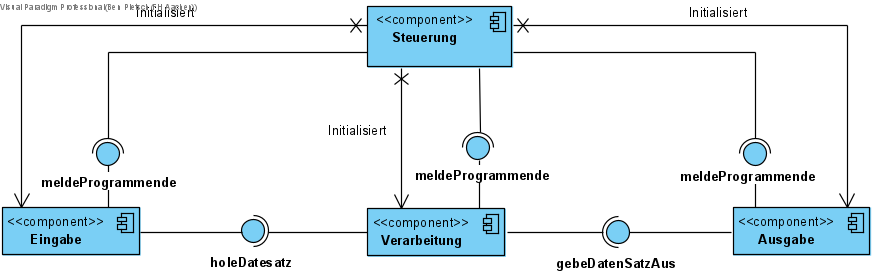
\includegraphics[width=\linewidth]{images/ComponentDiagram1}
    \caption{
        Komponentendiagramm, das die Kommunikation der Komponenten visualisiert.
    }
    \label{fig:komoponent}
\end{figure}


\section{Mathematische Beschreibung der vier Algorithmen}\label{sec:mat-beschreibung}
Die Verarbeitung wird jeweils auf einem einzelnen Datensatz aus der Eingabe durchgeführt.
Dieser Datensatz kann beschrieben werden durch eine Liste aus $N$ Datenpunkten, die jeweils einen \~x- und einen y-Wert beinhalten.
Aus den Datenpunkten wird in vier Verarbeitungsschritten das gewünschte Ergebnis gewonnen.

\subsection{Umrechnung und Normierung der Daten}\label{subsec:umrechnung-und-normierung}
Im ersten Schritt werden sowohl die \~x-Werte, als auch die y-Werte manipuliert.

Die y-Werte werden normiert, indem jeder einzelne y-Wert durch den maximalen y-Wert geteilt wird.
Also setzte $y_{max} = max(\bm{y})$ und berechne
\[
    y_k = \frac{y_k}{y_{max}}, \forall k \in [0, N - 1]
\]
Dafür werden zwei einfache Iterationen über die Datenliste benötigt:
Die erste zum Bestimmen des maximalen y-Wertes und die zweite um jeden y-Wert mit dem Maximum zu skalieren.

Jeder \~x-Wert wird durch die folgende Transformation in die Einheit Pikosekunden [ps] umgerechnet:
\[
    \tilde{x}_k = \frac{\tilde{x}_k}{2^{18} - 1} \cdot 266.3 - 132.3, \forall k \in [0, N - 1]
\]
Dieser Schritt benötigt lediglich eine Iteration und kann parallel zur zweiten Iteration der y-Normierung durchgeführt werden.

\subsection{Glättung der Daten}\label{subsec:glaettung}
Aufgrund von Messungenauigkeiten liegen die Sensordaten nicht in stetiger Form vor (siehe Abbildung~\ref{fig:glaettung}).
Deshalb wird nun jeder der \~x-Werte durch einen gleitenden Mittelwert aus seiner Umgebung ersetzt.
Für den gleitenden Mittelwert wird jedes Mal ein arithmetisches Mittel aus \~x-Werten in einem Intervall bestimmt.
Die Details dieser Berechnung werden nun genauer erläutert.

Im ersten Schritt wird die Breite des Intervalls festgelegt.
Diese hängt von der Anzahl der Datenpunkte $N$ ab.
\[
    n =
    \begin{cases}
        \lfloor0.002 \cdot N \rfloor - 1 & , \text{wenn} \lfloor0.002 \cdot N \rfloor \text{gerade} \\
        \lfloor0.002 \cdot N \rfloor     & , \text{wenn} \lfloor0.002 \cdot N \rfloor \text{ungerade}
    \end{cases}
\]
Diese Breite wird nun halbiert, und gibt die distanz in jeweils eine x-Richtung an.
\[
    \tau = \frac{n - 1}{2}
\]
Nun wird mit folgender Formel der gleitende Mittelwert für alle $N$ Datenpunkte berechnet.
\[
    x_k = \frac{1}{n} \sum_{i = 0}^{n - 1} \tilde{x}_{k-\tau+i}
\]
Für einen Punkt $k$ werden jeweils die $\tau$ vorherigen \~x-Werte, die $\tau$ nachfolgenden \~x-Werte und der aktuelle Wert an der Stelle $k$ aufaddiert.
Diese Summe wird dann durch die Anzahl der Summanden geteilt.
Wenn das für alle $N$ gemacht wurde, kann im Graph eine Glättung erkannt werden (siehe Abbildung~\ref{fig:glaettung}).

Bei der Berechnung des gleitenden Mittelwertes muss an den Rändern der Datenliste besonders Acht gegeben werden.
Gilt für den Index $k-\tau+i < 0$ oder $k-\tau+i > N + 1$, dann kann hier kein \~x-Wert zugeordnet werden.
Ein solcher Fall tritt z.B. auf, wenn $x_0$ berechnet werden soll.
Dann ist es sinnvoll den Mittelwert aus allen Punkten im Intervall zu bilden, bei denen ein \~x-Wert zugeordnet werden kann.
Da dadurch die Anzahl der Summanden geringer sein kann, muss der skalierende Faktor $\frac{1}{n}$ natürlich angepasst werden.


\begin{figure}[htb]
    \centering
    \begin{minipage}{.5\textwidth}
        \centering
        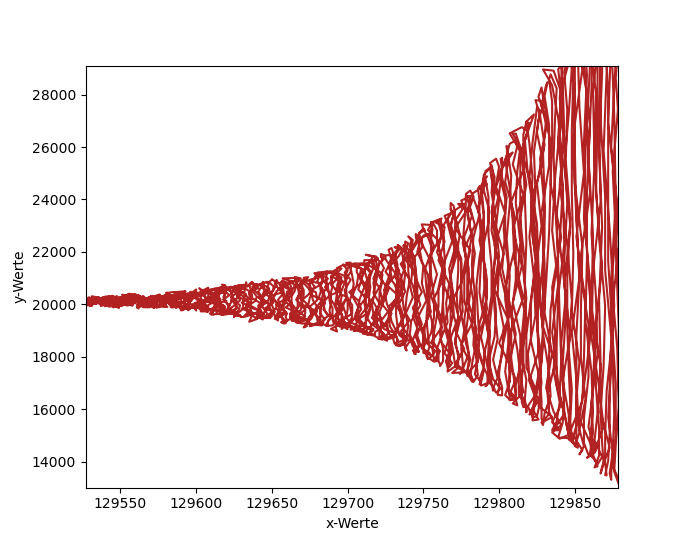
\includegraphics[width=\linewidth]{images/EingabeNichtGlatt}
    \end{minipage}%
    \begin{minipage}{.5\textwidth}
        \centering
        \includegraphics[width=\linewidth]{images/Geglättet}
    \end{minipage}
    \caption{Ausschnitt des eines Datensatzes vor (links) und nach (rechts) Skalierung, Normierung und Glättung.}
    \label{fig:glaettung}
\end{figure}


\subsection{Obere Einhüllende}\label{subsec:ober-einh}
Es soll nun eine Funktion bestimmt werden, die die gegebenen Daten nach oben hin abschätzt.
Diese wird für spätere Berechnungen benötigt.
Die Funktion wird als Feld der länge $N$ gespeichert.
Eine solche Funktion kann durch Bestimmen von lokalen Maxima bestimmt werden, was aber recht aufwändig ist.
Unter der Annahme, dass die Eingabedaten immer die Glockenform wie in Abbildung~\ref{fig:eingabe-plot} haben, kann die obere Einhüllende durch eine einfachere Methode approximiert werden.
\begin{figure}[htb]
    \centering
    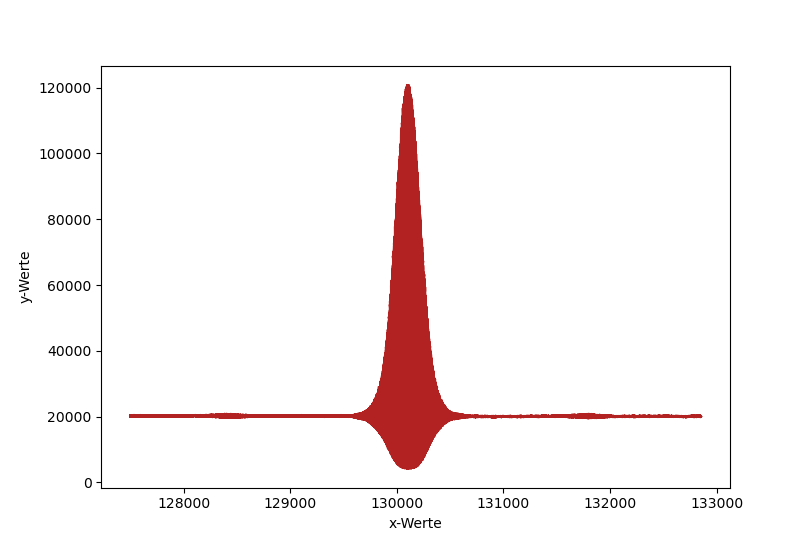
\includegraphics[width=0.8\linewidth]{images/EingabeInsgesamt}
    \caption{
        Ein Plot eines Datensatzes aus der Eingabe.
    }
    \label{fig:eingabe-plot}
\end{figure}

Im ersten Schritt werden wieder der maximale y-Wert (durch die Normierung sollte dieser nun 1 sein) und sein zugehöriger Index berechnet.

Dann wird vom Anfang der Liste der Datenpunkte (also grafisch von links aus) bis zum Index des Maximums iteriert.
In jedem Iterations-Schritt wird ein Wert der oberen Einhüllenden geschrieben.
Bei diesem Wert handelt es sich wieder um ein y-Maximum, das dynamisch während der Iteration gebildet wird.
Initial hat dieses lokale Maximum den Wert $y_0$.
Jedes Mal, wenn ein höherer y-Wert gefunden wird, überschreibt dieser das lokale Maximum.
Wenn der Index des Maximums erreicht wurde, kann die gleiche Methode vom anderen Ende der Liste wiederholt werden.
Dort wird also das lokale Maximum initial auf $y_{N-1}$ gesetzt.

Zuletzt darf nicht vergessen werden den Wert $y_{max}$ an der zugehörigen stelle in der oberen Einhüllenden einzutragen.

\begin{figure}[htb]
    \centering
    \begin{minipage}{.5\textwidth}
        \centering
        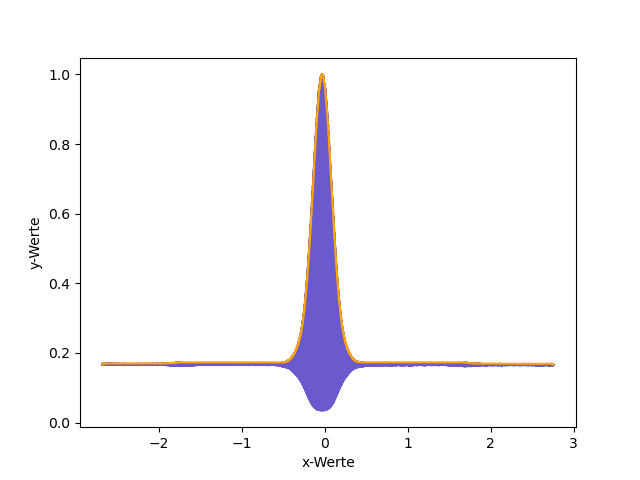
\includegraphics[width=\linewidth]{images/ObereEinhuellende}
    \end{minipage}%
    \begin{minipage}{.5\textwidth}
        \centering
        \includegraphics[width=\linewidth]{images/EinhüllendeNah}
    \end{minipage}
    \caption{Die obere Einhüllende, erstellt durch das beschriebene Verfahren.}
    \label{fig:oberer-einh}
\end{figure}

\subsection{Pulsbreite}\label{subsec:pulsbreite}
Im letzten Schritt der Verarbeitung soll die Pulsbreite berechnet werden.

Zuerst muss dazu die Grundlinie berechnet werden.
Diese berechnet sich als arithmetisches Mittel der y-Werte aus den ersten 1\% der Messpunkte in der Liste.
Also setze
\[
    n = \lfloor0.01 \cdot N \rfloor
\]
und
\[
    Grundlinie = \frac{1}{n} \sum_{k = 0}^{n - 1} y_k
\]
Im Anschluss wird wieder der maximale y-Wert benötigt, um den Punkt auf halber Höhe von Grundlinie zum Maximum zu ermitteln.
\[
    Zielwert = \frac{y_{max} - Grundlinie}{2} + Grundlinie
\]
Nun wird jeweils von links und von rechts aus der erste Messpunkt gesucht, bei dem der y-Wert den Zielwert übersteigt.
Das kann durch zwei einfache Iterationen über die Datenliste umgesetzt werden.
Die Indizes dieser beiden Punkte werden gespeichert als $L$ für den Wert von links und als $R$ für den Wert von rechts.
Die Pulsbreite berechnet sich jetzt durch die x-Werte der beiden Datenpunkte.
\[
    Pulsbreite = x_R - x_L
\]

\begin{figure}[htb]
    \centering
    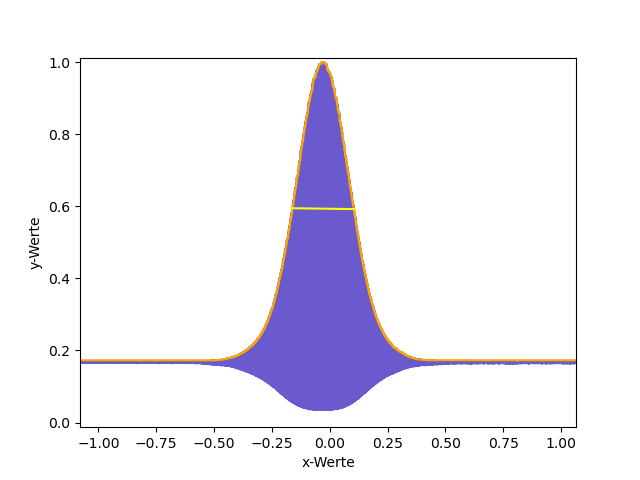
\includegraphics[width=0.7\linewidth]{images/Pulsbreite}
    \caption{
        Die Pulsbreite eines verarbeiteten Datensatzes (die Länge der Gelben Linie).
    }
    \label{fig:pulsbreite}
\end{figure}


\section{Gesamtsystem}\label{sec:gesamtsystem}

\subsection{Eingabe}\label{subsec:eingabe}

\subsection{Verarbeitung}\label{subsec:verarbeitung}

\subsection{Ausgabe}\label{subsec:ausgabe}

\subsection{Datenstrukturen}\label{subsec:datenstrukt}
